\documentclass[12pt,oneside,french]{article}
\usepackage[utf8]{inputenc}
\usepackage[T1]{fontenc}
\usepackage[french]{babel}
    \DecimalMathComma
    \parindent=0cm
\usepackage{lmodern}
    \renewcommand{\familydefault}{\sfdefault}
\usepackage[a4paper]{geometry}
    \geometry{verbose,tmargin=1.5cm,bmargin=1.5cm,lmargin=1.5cm,rmargin=1.5cm}
\usepackage{amsmath}
\usepackage{amssymb}
\usepackage{eurosym}
    \newcommand{\var}[1]{\textbf{\texttt{#1}}}
    \newcommand{\txt}[1]{\texttt{#1}}
\usepackage{enumerate}
\usepackage{multicol}
\usepackage[table]{xcolor}
\usepackage{tikz}
\usepackage[tikz]{bclogo}
\usepackage{tabularx}
\usepackage{ulem}
\usepackage{hyperref}
    \hypersetup{
        colorlinks=true,
        linkcolor=black,
        filecolor=black,      
        urlcolor=blue,
    }

\renewcommand{\thesection}{\arabic{section}.}

\newcounter{exo}
\renewcommand{\theexo}{\arabic{notp}.\arabic{exo}}
\newenvironment{exo}
    {\refstepcounter{exo}\begin{bclogo}[couleurBord=black!50,arrondi=0.3,barre=none,logo=\bccrayon,nobreak]{\textbf{~Exercice \theexo}}}
    {\end{bclogo}}
\newenvironment{exo2}
    {\refstepcounter{exo}\begin{bclogo}[couleurBord=black!50,arrondi=0.3,barre=none,logo=\bccrayon]{\textbf{~Exercice \theexo}}}
    {\end{bclogo}}

\newcounter{notp}
\newcommand{\tp}[1]{\stepcounter{notp} \setcounter{exo}{0}\setcounter{section}{0} \begin{center}{\huge TP Python \no\thenotp~: #1}\end{center}}

\newcommand{\exemple}{\textbf{\textsf{Exemple}}}
\newcommand{\comment}[1]{{\color{blue} \# #1}}
\newcommand{\bcpython}{\hspace{-8.5pt}
\includegraphics[width=17pt]{python.png}}
\newenvironment{python}
    {\begin{center}{\color{blue!60}\vrule width 1.5pt}\bcpython\begin{minipage}[t]{15cm}\ttfamily}
    {\par\end{minipage}\end{center}\smallskip}

\newcommand{\interligne}{\rule[-8pt]{0pt}{25pt}}
\newcommand{\pointilles}{\noindent \interligne \dotfill}
\newcommand{\reponse}[2]{\interligne \ifthenelse{\equal{#1}{c}}{\dotfill}{}{\color{blue}#2} \dotfill}
\newcommand{\minireponse}[1]{\makebox[1cm]{\interligne{\color{blue}#1}}}

\begin{document}
\large

\setcounter{section}{0}
\begin{center}{\huge Ouvrir une interface Python}\end{center}

Python est un langage de programmation fonctionnant sur la plupart des plates-formes informatiques.
Au lycée, nous utiliserons la version 3 de Python, dont la syntaxe de certaines commandes diffère légèrement de la version 2.\\
Pour utiliser Python, on utilise souvent un environnement de développement intégré (\texttt{IDE}) tel qu'\texttt{IDLE}. On peut aussi trouver un interpréteur en ligne sur internet, comme par exemple le site \texttt{Replit.com}.

\section{\texttt{IDLE}}

Au lancement d'\texttt{IDLE}, apparaît une seule fenêtre. C'est dans celle-ci que s'afficheront les sorties du programme.\medskip

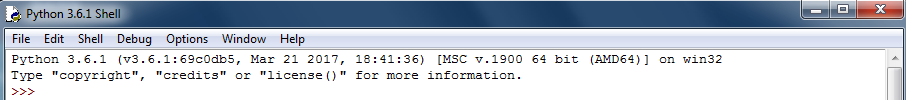
\includegraphics[width=\linewidth]{IDLEsorties.png}

Le programme doit être écrit dans une seconde fenêtre. Pour l'obtenir il faut cliquer sur \fbox{File} puis \fbox{New File}. Exemple :\medskip

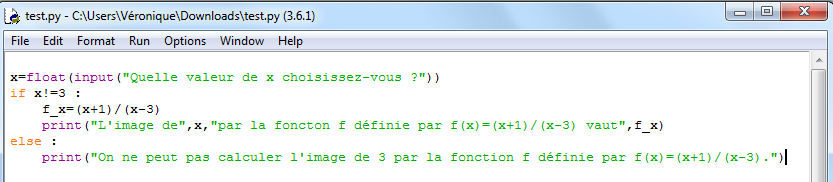
\includegraphics[width=\linewidth]{IDLEprog.png}

Pour exécuter le programme, il faut cliquer sur \fbox{Run} puis \fbox{Run Module} et aller voir le résultat dans la première fenêtre :\medskip

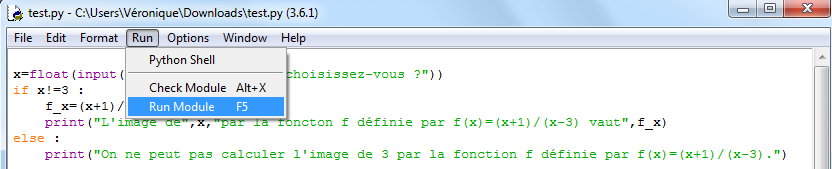
\includegraphics[width=\linewidth]{IDLErun.png}
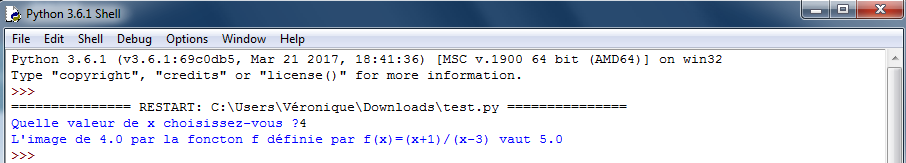
\includegraphics[width=\linewidth]{IDLEout.png}

\section{\texttt{replit.com}}

Le site internet \texttt{\url{https://replit.com/}} permet d'exécuter des programme en Python directement en ligne sans aucune installation. Depuis peu, une inscription gratuite est necessaire. Cette solution est recommandée à la maison car elle permet d'utiliser Python sans rien n'installer et permet aussi de retrouver son travail depuis le lycée. En classe, \texttt{IDLE} reste recommandé car il offre les meilleurs performances.

Le programme est tapé dans la partie gauche. En cliquant sur \fbox{Run} les résultats s'afficheront sur la partie droite comme dans l'exemple :\medskip

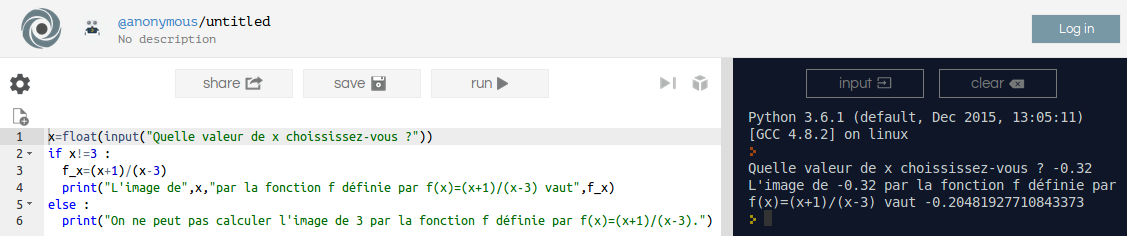
\includegraphics[width=\linewidth]{replit.png}

Remarque : \texttt{\url{https://replit.com/}} permet aussi de travailler avec les autres langages abordés ce trimestre (HTML, CSS, JavaScript par exemple).

\end{document}
